\chapter{Algoritmo de Grover}
%El algoritmo de Grover es un AC que encuentra con alta probabilidad la entrada única de una función de caja negra que produce un valor particular de salida, usando tan sólo $O(\sqrt{N})$ evaluaciones de la función, donde $N$ es el tamaño del dominio de la función. El análogo clásico de este algoritmo requiere $O(N)$ evaluaciones de la función, pues, el elemento correcto podría ser el $N$-ésimo en ser evaluado y se deben evaluar uno por uno. La aplicación directa de este algoritmo es como algoritmo de búsqueda en una base de datos. Sin embargo, su aplicación más eficiente es como subrutina en diversos procesos de optimización.

El algoritmo de Grover es un AC que realiza una búsqueda en una secuencia no ordenada de datos con $N=2^n$ entradas. Clásicamente esta búsqueda tendría un orden de complejidad de $O(N)$, pues, como los datos no están ordenados, la cantidad promedio de evaluaciones que se deben realizar crece linealmente con la cantidad de entradas. En el caso del algoritmo de Grover, la complejidad de la búsqueda es de $O(\sqrt{N})$, pues se requieren aproximadamente $\frac{\pi\sqrt{N}}{4}$ iteraciones para hallar la entrada deseada. En cuanto a la cantidad de qubits requeridos, se necesitan $O(\log_2 N)$ qubits, pues se debe realizar un estado superpuesto donde cada componente de la superposición represente una entrada de la secuencia de datos.

Introducción:

Dada $f:{0,1}^n \rightarrow {0,1}$, es decir; $f:{0,1,2,...,N-1} \rightarrow
{0,1}$, se tiene la promesa de que 
\[
  f(x) = 
\begin{cases}
1 & \text{si } x = x_0 \\
0 & \text{si } x \neq x_0
\end{cases}
\]

Hay que determinar $x$.

Clásicamente hay que evaluar la función $N=2^n$ veces. Cuánticamente sólo se
requiere evaluar $\sqrt{2^n}$ veces.

El análisis usual del algoritmo de Grover se basa en un hecho bien conocido de
la geometría plana elemental: ``El producto de dos reflexiones es una rotación''

Veamos qué significa esto:

Supongamos que tenemos el oráculo

\[U_f \ket{x} = (-1)^{f(x)} \ket{x} =
    \begin{cases}
      \ket{x} & \text{si } x \neq x_0 \\
      - \ket{x} & \text{si } x = x_0
    \end{cases}\]

Es decir: $U_f = \mathds{1} - 2 \ketbra{x_0}{x_0}$
  
El efecto de $U_f$ es invertir la componente de $\ket{\phi}$ en la dirección
$\ket{x_0}$.

Además, podemos definir otro operador unitario $U_s = -\mathds{1} + 2
\ketbra{s}{s}$ donde $\ket{s} = H^{\otimes n} \ket{0} = \frac{1}{\sqrt{2^n}}
\sum\limits_x \ket{x}$

El efecto de $U_s$ es invertir todas las componentes en direcciones
perpendiculares a $\ket{s}$. Es decir, refleja respecto de $\ket{s}$.

Hagamos ahora el siguiente ejercicio:

Cosidremos el estado inicial $\ket{\psi}$

\begin{enumerate}
\item Aplicamos $U_\omega$, que invierte la componente $\ket{x_0}$.
\item Aplicamos $U_s$, que refleja respecto de $\ket{s}$
\end{enumerate}

La combinación de estas dos inversiones es una rotación en un ángulo $2\alpha$.

%%%%%% INSERTAR GRÁFICAS DEL EJEMPLO %%%%%%

Una vez entendido esto empecemos el algoritmo de Grover.

Algoritmo de Grover:

Asumamos que el tamaño de nuestra base de datos es $2^n \equiv N$, donde $n$ es cualquier número entero distinto de creo.

Consideremos un observable $\Omega \in H$ de dimensión $N \geq 2$. Este
observable define un conjunto de bases ortogonales $\ket{x} = \{\ket{0},
\ket{1}, \ket{2},...,\ket{N-1}\}$ con autovalores conocidos $\lambda_0,
\lambda_1, \lambda_2,..., \lambda_{N-1}$, tal que $\hat{\Omega} \ket{j} =
\lambda_j \ket{j}$, $j \in {0,...,N-1}$.

Entonces podemos asociar un único autoestado $\ket{x_j}$, o autovalor
$\lambda_j$, con cada item en la base de datos.

El problema de buscar en la base de datos se convierte ahora en el problema de
medir un autovalor de interés al que llamaremos $\lambda_\omega$, asociado con
el estado $\ket{\omega}$, el cual representa algún específico item $\omega$ en
nuestra base de datos y el cuál deseamos encontrar usando el algoritmo de
búsqueda de Grover.

Entonces:

$$\{\ket{x}\}_{x=0,1,...,N-1} \text{es ortonormal }\rightarrow \ket{s} =
\frac{1}{\sqrt{N}} \sum\limits_{x=0}^{N-1} \ket{x} = \text{autoestado asociado a
  la base de datos}$$

$$\braket{s}{s} = 1 \text{ ya que } \braket{i}{j} = \delta_{ij}$$

Cualquier autoestado $\ket{\omega}$ tiene la misma proyección
$\braket{\omega}{s} = \frac{1}{sqrt{N}}$, y dado un item $\omega$ la
probabilidad de medir $\lambda_\omega$ (que es equivaletne a encontrar $\ket{s}$
en el estado $\ket{\omega}$) es $|\braket{\omega}{s}|^2 = \frac{1}{N}$,
consistentemente con lo que ocurre con una base de datos clásica.

Consideremos ahora el oráculo unitario $U_\omega$ definido como:

$$U_\omega \equiv \mathds{1} - 2\ketbra{\omega}{\omega}$$

Entonces $U_\omega \ket{x} = (\mathds{1} - 2\ketbra{\omega}{\omega}) \ket{x} =
\ket{x} - 2 \braket{\omega}{x} \ket{\omega} = \ket{x} - 2 \delta_{ij} \ket{\omega}$
 Si $x \neq \omega \rightarrow U_\omega \ket{x} = \ket{x}$ 
 Si $x = \omega \rightarrow U_\omega \ket{x} = -\ket{\omega}$ 

De manera tal que $U_\omega \ket{s} = U_\omega (\frac{1}{\sqrt{N}}
\sum\limits_{x = 0}^{N-1}) = \frac{1}{\sqrt{N})} U_\omega (\sum\limits_{x=0,
  x\neq\omega}^{N-1} \ket{x} + \ket{\omega}) =
\frac{1}{\sqrt{N}}\sum\limits_{x=0, x\neq\omega}^{N-1} \ket{x} -
\frac{1}{\sqrt{N}} \ket{\omega}$.

Esto se puede reescribir como:

$U_\omega \ket{s} = \frac{1}{\sqrt{N}} \sum\limits_{x=0, x\neq\omega}^{N-1}
\ket{x} + (\frac{1}{\sqrt{N}} \ket{\omega} - \frac{1}{\sqrt{N}} \ket{\omega} )- \frac{1}{\sqrt{N}} \ket{\omega} $

Por lo tanto: $U_\omega \ket{s} = \frac{1}{\sqrt{N}} \sum_{x=0}^{N-1} \ket{x} -
\frac{2}{\sqrt{N}} \ket{\omega} \rightarrow U_\omega \ket{s} = \ket{s} -
\frac{2}{\sqrt{N}} \ket{\omega}$

Llamemos $\ket{\psi} \equiv U_\omega \ket{s} = \ket{s} - \frac{2}{\sqrt{N}} \ket{\omega}$
como $0 \leq \braket{s}{\psi} \leq 1$

llamemos $\cos(\theta) \equiv \braket{s}{\psi} \equiv \braket{s}{s} -
\frac{2}{\sqrt{N}} \braket{s}{\omega} = 1 - \frac{2}{\sqrt{N}}
\frac{1}{\sqrt{N}} \rightarrow \cos(\theta) = 1 - \frac{2}{N}$

cuando $N$ es grande $\cos(\theta) \approx 1$ pero nunca es uno

Cosideremos ahora un segundo operador $U_s$ definido como:

$U_s = 2 \ketbra{s}{s} - \mathds{1}$

Se define el operador de Grover como $G = U_s U_\omega$

Consideremos la iteración de Grover $\ket{\psi_1} \equiv G \ket{s} \rightarrow
\ket{\psi_1} = U_s U_\omega \ket{s} = U_s \ket{\psi}$

luego: $\ket{\psi_1} = U_s \ket{\psi} = U_s (\ket{s} - \frac{2}{\sqrt{N}} \ket{\omega})$

$\ket{\psi_1} = 2 \braket{s}{s} \ket{s} - \ket{s} - \frac{4}{\sqrt{N}}
\braket{s}{\omega} \ket{s} + \frac{2}{\sqrt{N}} \ket{\omega} $

$\ket{\psi_1} = \ket{s} - \frac{4}{N} \ket{s} + \frac{2}{\sqrt{N}} ket{\omega} $

$\ket{\psi_1} = (1-\frac{4}{N}) \ket{s} + \frac{2}{\sqrt{N}} \ket{\omega} $

La acción de G sobre $\ket{s}$ incrementa la amplitud de probabilidad del
autoestado de componente $\ket{\omega}$, después de la rotación.

El correspondiente ángulo de rotación $\theta^\prime$ viene dado por:

$\cos(\theta^\prime) = \braket{s}{\psi} = \bra{s} [(1-\frac{4}{N})\ket{s} +
\frac{2}{\sqrt{N}} \ket{\omega}] =
(1-\frac{4}{N}+\frac{2}{\sqrt{N}}\frac{1}{\sqrt{N}}) = 1 - \frac{2}{N} = \cos(\theta)$

Por lo tanto $\cos(\theta^\prime) = \cos(\theta)$

Confirmando así que los ángulos de rotación $\theta^\prime$ y $\theta$ debidos a
la acción de $G$ y $U_\omega$ son iguales en valor absoluto. De hecho, rotando
el mismo ángulo $\theta = \theta^\prime$ en valor absoluto, en direcciones
opuestas sobre $\ket{s}$ se forma un ángulo $\theta^{\prime \prime} = 2 \theta$.

$\cos(\theta^{\prime\prime}) = \braket{\psi}{\psi_1} = [\bra{s} -
\frac{2}{\sqrt{N}} \bra{\omega}][(1-\frac{4}{N})\ket{s}+\frac{2}{\sqrt{N}}
\ket{\omega}] = (1-\frac{4}{N})\braket{s}{s} -
\frac{2}{\sqrt{N}}(1-\frac{4}{N})\braket{\omega}{s} + \frac{2}{\sqrt{N}}
\braket{s}{\omega} - \frac{2}{\sqrt{N}}\frac{2}{\sqrt{N}}
\braket{\omega}{\omega} = 1 - \frac{4}{N} -
\frac{2}{\sqrt{N}}(1-\frac{4}{N})\frac{1}{\sqrt{N}} +
\frac{2}{\sqrt{N}}\frac{1}{\sqrt{N}} - \frac{4}{N} = 1 - \frac{8}{N} +
\frac{8}{N^2} = 2(1-\frac{2}{N})^2 -1 = 2 \cos^2(\theta) -1 = \cos(2\theta)$

Por lo tanto: $\theta^{\prime\prime} = 2\theta$

La relación entre los estados $\ket{s}, \ket{\psi}, \ket{\psi_1}$ y $\ket{\omega}$
y sus relaciones de proyección $\braket{\omega}{s}$ y $\braket{\omega}{\psi_1}$
son ilustradas en la siguiente figura

Como recordamos $\hat{\Omega}\ket{j} = \lambda_j \ket{j} \qquad j \in
\{0,1,...,N-1\}$ y $\omega \in {0,1,...,N-1}$.

$\hat{\Omega} \ket{\omega} = \lambda_\omega \ket{\omega}$

Luego si realizamos una medida en el estado $\ket{\psi_1}$ con el observable
$\hat{\Omega}$, la probabilidad de medir $\lambda_\omega$ es:

$|\braket{\omega}{\psi_1}|^2 = |\bra{\omega} [(1-\frac{4}{N})\ket{s} +
\frac{2}{\sqrt{N}} \ket{\omega}]|^2 = \frac{1}{N}(3-\frac{4}{N})^2 = \frac{1}{N}
(9 - \frac{24}{N} + \frac{16}{N^2})$

$\lim_{N \to \text{grande}} |\braket{\omega}{\psi_1}|^2 \approx \frac{9}{N}$

Este resultado muestra que una simple interacción de Grover y su respectiva
medida aumenta casi en 9 veces el valor de la probabilidad clásica.

Grover $\approx \frac{9}{N}$ Medida clásica $= \frac{1}{\sqrt{N}}$

Siguiendo el mismo esquema, podemos aplicar el operador de Grover varias veces
rotando el sistema lo más cercano posible del estado $\ket{\omega}$
incrementando así la probabilidad de medir $\lambda_\omega$ con la precisión
requerida.

El efecto producido por los operadores unitarios $U_\omega$ y $G$ sobre el
estado inicial se ilustra en la siguiente figura.

%%%%%% FIGURE HERE %%%%%%

Para derivar una fórmula de iteración, redefinamos el autoestado original
$\ket{s}$ quitándole el estado $\ket{\omega}$ de la serie, es decir:

$\ket{u} \equiv \frac{1}{\sqrt{N-1}} \sum\limits_{x=0, x\neq\omega}^{N-1}
\ket{x} = \sqrt{\frac{N}{N-1}} \ket{s} - \frac{1}{\sqrt{N-1}} \ket{\omega}$

Entonces podemos reescribir $\ket{s}$ en términos de $\ket{\omega}$, tal que:

$\ket{s} = \frac{1}{N} \sum\limits_{x=0}^{N-1} \ket{x} \equiv
\sqrt{1-\frac{1}{N}} \ket{u} + \frac{1}{\sqrt{N}} \ket{\omega}$

como $0\leq \sqrt{1-\frac{1}{N}} \leq 1, 0\leq \frac{1}{\sqrt{N}} \leq 1$ y
$(\sqrt{1-\frac{1}{N}})^2 + (\frac{1}{\sqrt{N}})^2 = 1$

podemos asociar: $\cos(\frac{\theta}{2}) = \sqrt{1-\frac{1}{N}}$ y
$\sin(\frac{\theta}{2}) = \frac{1}{N}$

quedándonos $\ket{s} = \cos({\theta}{2}) = \sqrt{1-\frac{1}{N}}$

Se puede demostrar que si aplicamos k veces el operador de Grover se obtiene:

$G^k \ket{s} = \cos((2k+1)\frac{\theta}{2}) \ket{u} +
\sin((2k+1)\frac{\theta}{2}) \ket{\omega}$

Este resultado muestra que después de k iteraciones del operador de Grover, el
estado inicial $\ket{s}$ rota un ángulo $k\theta$.

%%%%%% DIBUJO AQUÍ %%%%%%

La probabilidad $p(\omega)$ de encontrar el estado $G^k \ket{s}$ en
$\ket{\omega}$, y por ende la medida del autovalor $\lambda_\omega$ con el
observable $\hat{\Omega}$ está dada por

$p(\omega) = |\bra{\omega} G^k \ket{s}|^2 = \sin^2((2k+1)\frac{\theta}{2})$

Esta probabilidad alcanza un máximo cuando $\sin^2((2k+1)\frac{\theta}{2}) = 1$,
y eso ocurre cuando $k_{max} \theta + \frac{theta}{2} = \frac{\pi}{2}
\rightarrow k_{max} = \frac{\pi-\theta}{2\theta}$

por otro lado, ya vimos que $\sin(\frac{\theta}{2}) = \frac{1}{\sqrt{N}}$, y si
N es grande $\theta$ se hace pequeño

$\sin(\frac{theta}{2}) \approx \frac{\theta}{2} - \frac{(\theta/2)^3}{3!} + ...
\approx \frac{\theta}{2} = \frac{1}{\sqrt{N}} \rightarrow \theta \approx \frac{2}{\sqrt{N}}$

$k_{max} = \frac{\pi}{2\theta} - \frac{\theta}{2\theta} \approx \frac{\pi}{2
  \frac{2}{\sqrt{N}}} - \frac{1}{2} \approx \frac{\pi}{4} \sqrt{N} - \frac{1}{2}
\rightarrow k_{max} \approx \frac{pi}{4} \sqrt{N} = O(\sqrt{N})$

El algoritmo de Grover debe detenerse cuando $k \approx k_{max}$ ya que en dicho
caso $p(\omega) \approx 1$ y ya hemos encontrado el estado $\ket{\omega}$
deseado.

Esto se ilustra mejor en la siguiente figura:

%%%%%% FIGURA %%%%%%

Esta figura es muy importante ya que en ella se muestra la probabilidad en
función del número de iteraciones, desde bases de datos cuyos tamaños van desde
$N = 2^6 = 64$ hasta $N = 2^{14} = 16384$

Debido a la dependencia de Grover del $O(\sqrt{N})$ encontramos que en el caso
clásico con $N = 2^{14} = 16384$ iteraciones en Grover solo tenemos $k_{max}
\approx 100$ iteraciones de Grover.

En resumen:

Algoritmo Clásico $\rightarrow$ 16384 iteraciones
Algoritmo de Grover $\rightarrow \approx$ 100 iteraciones

\subsection{Implementación circuital del algoritmo de Grover}

Consideremos como ejemplo $\implies N = s^3 = 8$, luego:

1)

$\ket{s} = \frac{1}{\sqrt{N}} \sum\limits_{x=0}^{N-1} \ket{x} = H^{\otimes n}
\ket{0} = \ket{+}^{\otimes n}$

Si: $N = 2^3 = 8$

$\ket{s} = \frac{1}{\sqrt{2^3}} \sum\limits_{x=0}^{7} \ket{x} = H^{\otimes 3}
\ket{0} = \frac{1}{2^3} (\ket{000} + \ket{001} + \ket{010} + \ket{011} + \ket{100} + \ket{101} + \ket{110} + \ket{111})$

En resumen, necesitamso una ancilla $\ket{0}$ y $n$ compuertas de Hadamard para
crear $\ket{s}$.

2)

Necesitamos crear el operador $U_\omega$, ``el oráculo''.

$U_\omega \ket{x} = -\ket{\omega}$ si $x = \omega$
$U_\omega \ket{x} = \ket{x}$ si $x \neq \omega$

Además, si $x = \{0, 1, ... , N-1\} \implies \begin{cases} f(x) = 1 \text{ si }
  x = \omega \\ f(x) = 0 \text{ si } x \neq \omega \end{cases}$














\section{El operador de difusión de Grover}

\begin{figure}[H]
\centering 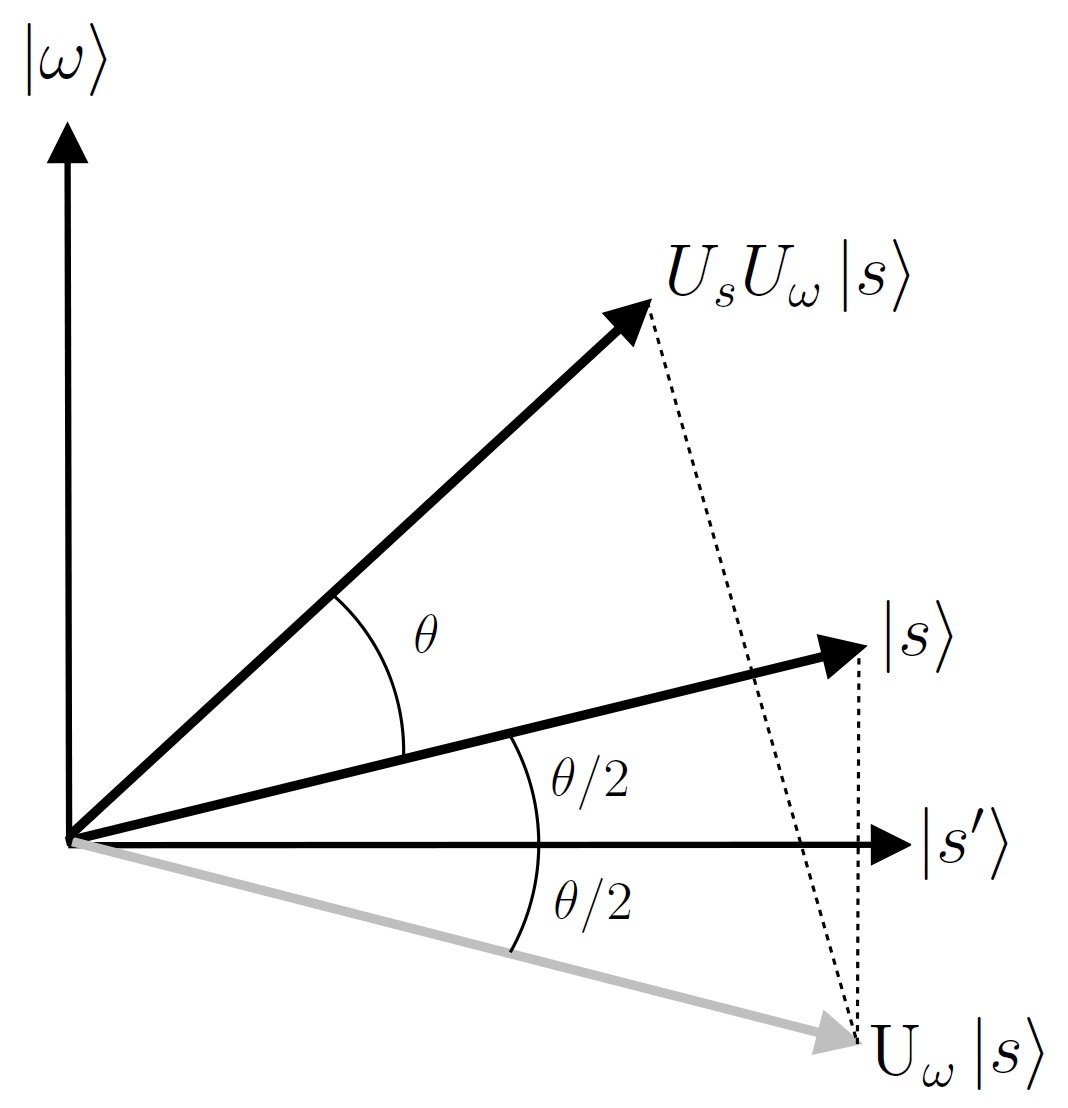
\includegraphics[width=0.3\linewidth]{img/grover_geometry.png}
\caption{Interpretación geométrica del operador difusión}
\end{figure}

$U_s = 2 \ket{s} \bra{s} - I$

$U_{\omega} = I - 2 \ket{\omega} \bra{\omega}$

\section{El algoritmo}

\[
\Qcircuit @C=1.4em @R=1.8em {
\lstick{\ket{0}} & {/^n} \qw & \gate{H^{\otimes n}} & \multigate{1}{U_{\omega}} & \gate{U_s} & \meter & \cw \\
\lstick{\ket{1}} & \qw & \gate{H} & \ghost{U_{\omega}} & \qw & \qw & \qw \\
& & & \rstick{\hspace{-13pt} \frac{\pi}{4} \sqrt{N} \text{ veces}}
\gategroup{1}{4}{2}{5}{1.8em}{_\}}
}
\]

\begin{enumerate}
\item Inicializar el estado del sistema.
\item Aplicar la transformada de Walsh-Hadamard.
\item Realizar la iteración de Grover $\lfloor \frac{\pi}{4} \sqrt{N} \rfloor$ veces.
\begin{enumerate}
\item Aplicar $U_{\omega}$.
\item Aplicar $U_s$.
\end{enumerate}
\item Realizar la medida $\Omega$.
\end{enumerate}



